% Options for packages loaded elsewhere
\PassOptionsToPackage{unicode}{hyperref}
\PassOptionsToPackage{hyphens}{url}
\PassOptionsToPackage{dvipsnames,svgnames*,x11names*}{xcolor}
%
\documentclass[
  11pt,
]{article}
\usepackage[]{mathpazo}
\usepackage{amsmath}
\usepackage{ifxetex,ifluatex}
\ifnum 0\ifxetex 1\fi\ifluatex 1\fi=0 % if pdftex
  \usepackage[T1]{fontenc}
  \usepackage[utf8]{inputenc}
  \usepackage{textcomp} % provide euro and other symbols
  \usepackage{amssymb}
\else % if luatex or xetex
  \usepackage{unicode-math}
  \defaultfontfeatures{Scale=MatchLowercase}
  \defaultfontfeatures[\rmfamily]{Ligatures=TeX,Scale=1}
\fi
% Use upquote if available, for straight quotes in verbatim environments
\IfFileExists{upquote.sty}{\usepackage{upquote}}{}
\IfFileExists{microtype.sty}{% use microtype if available
  \usepackage[]{microtype}
  \UseMicrotypeSet[protrusion]{basicmath} % disable protrusion for tt fonts
}{}
\makeatletter
\@ifundefined{KOMAClassName}{% if non-KOMA class
  \IfFileExists{parskip.sty}{%
    \usepackage{parskip}
  }{% else
    \setlength{\parindent}{0pt}
    \setlength{\parskip}{6pt plus 2pt minus 1pt}}
}{% if KOMA class
  \KOMAoptions{parskip=half}}
\makeatother
\usepackage{xcolor}
\IfFileExists{xurl.sty}{\usepackage{xurl}}{} % add URL line breaks if available
\IfFileExists{bookmark.sty}{\usepackage{bookmark}}{\usepackage{hyperref}}
\hypersetup{
  pdftitle={Data Science Project Guide: Airbnb},
  pdfauthor={TechAcademy e.V.},
  colorlinks=true,
  linkcolor=Maroon,
  filecolor=Maroon,
  citecolor=Blue,
  urlcolor=blue,
  pdfcreator={LaTeX via pandoc}}
\urlstyle{same} % disable monospaced font for URLs
\usepackage[top=0.5in, bottom=1.5in, left=1in, right=1in, a4paper]{geometry}
\usepackage{longtable,booktabs}
% Correct order of tables after \paragraph or \subparagraph
\usepackage{etoolbox}
\makeatletter
\patchcmd\longtable{\par}{\if@noskipsec\mbox{}\fi\par}{}{}
\makeatother
% Allow footnotes in longtable head/foot
\IfFileExists{footnotehyper.sty}{\usepackage{footnotehyper}}{\usepackage{footnote}}
\makesavenoteenv{longtable}
\usepackage{graphicx}
\makeatletter
\def\maxwidth{\ifdim\Gin@nat@width>\linewidth\linewidth\else\Gin@nat@width\fi}
\def\maxheight{\ifdim\Gin@nat@height>\textheight\textheight\else\Gin@nat@height\fi}
\makeatother
% Scale images if necessary, so that they will not overflow the page
% margins by default, and it is still possible to overwrite the defaults
% using explicit options in \includegraphics[width, height, ...]{}
\setkeys{Gin}{width=\maxwidth,height=\maxheight,keepaspectratio}
% Set default figure placement to htbp
\makeatletter
\def\fps@figure{htbp}
\makeatother
\setlength{\emergencystretch}{3em} % prevent overfull lines
\providecommand{\tightlist}{%
  \setlength{\itemsep}{0pt}\setlength{\parskip}{0pt}}
\setcounter{secnumdepth}{5}
\newcommand{\sectionbreak}{\clearpage}
\usepackage{booktabs}
\RequirePackage{fix-cm}
\usepackage[many]{tcolorbox}
\usepackage{xcolor}

\definecolor{r}{HTML}{2369bd}
\definecolor{p}{HTML}{ffde4d}
\definecolor{boxgrey}{HTML}{fefefe}

\newtcolorbox{rbox}{
  colback=boxgrey,
  colframe=r,
  coltext=black,
  boxsep=5pt,
  arc=4pt}
  
\newtcolorbox{pbox}{
  colback=boxgrey,
  colframe=p,
  coltext=black,
  boxsep=5pt,
  arc=4pt}


\newenvironment{tips}[1]
  {
  \begin{itemize}
  \footnotesize
  \renewcommand{\labelitemi}{
    \raisebox{-.7\height}[0pt][0pt]{
      {\setkeys{Gin}{width=3em,keepaspectratio}
        \includegraphics{images/#1.png}}
    }
  }
  \setlength{\fboxsep}{1em}
  \begin{rbox}
  \item
  }
  {
  \end{rbox}
  \end{itemize}
  }
  
  
\newenvironment{tipsp}[1]
  {
  \begin{itemize}
  \footnotesize
  \renewcommand{\labelitemi}{
    \raisebox{-.7\height}[0pt][0pt]{
      {\setkeys{Gin}{width=3em,keepaspectratio}
        \includegraphics{images/#1.png}}
    }
  }
  \setlength{\fboxsep}{1em}
  \begin{pbox}
  \item
  }
  {
  \end{pbox}
  \end{itemize}
  }
  
\usepackage{fancyhdr}
\pagestyle{fancyplain}
\usepackage{setspace}
\usepackage{chngcntr}
\onehalfspacing

\usepackage{titling}
\pretitle{\begin{center}\LARGE\includegraphics[width=6cm]{plots/TA_Logo.png}\\[\bigskipamount]}
\posttitle{\end{center}}
\ifluatex
  \usepackage{selnolig}  % disable illegal ligatures
\fi
\usepackage[]{natbib}
\bibliographystyle{apalike}

\title{Data Science Project Guide: Airbnb}
\author{TechAcademy e.V.}
\date{Winter Term 2020/21}

\begin{document}
\maketitle

\clearpage

\addtolength{\headheight}{17.82275pt}
\rhead{\includegraphics[height=0.5cm]{plots/TA_logo.png}}

\fancyfoot{}
\fancyfoot[R]{\thepage}
\addtolength{\headheight}{17.82275pt}

\fancyfoot[L]{Data Science Project Guide | Airbnb | \copyright\ 2020, TechAcademy e.V.}

\renewcommand{\headrulewidth}{0.25pt}
\renewcommand{\footrulewidth}{0.25pt}

\tableofcontents
\clearpage

\hypertarget{welcome}{%
\section{Welcome!}\label{welcome}}

In the first few chapters you will be introduced to the basics of the \texttt{R} and \texttt{Python} tracks respectively and you will find helpful explanations to questions you might have in the beginning of your coding journey. There will be a quick introduction to the Data Science track so that you can get started with the project quickly. So let's get started with the basics!

In all tracks you will work on your project in small groups of fellow students. This not only helps you get the project done faster, it also helps make your results even better. Our experience shows: The different backgrounds of the members and discussing different opinions and ideas will produce the best results. Besides, it is of course more fun to work on a project together than to code alone!\\
The groups can consist of a maximum of three members. You can choose your two teammates independently, we won't interfere with your arrangements. It is important that all group members complete the same level of difficulty (beginner or advanced), since the tasks are different in scope for each level. We explicitly encourage you to collaborate with students from different departments. This not only allows you to get to know people from other departments, but may even give you a whole new perspective on the project and tasks.
When submitting it is important to note: for a certificate, each person must submit the project individually. However, this can be identical within your group. You can get more information at our first Coding Meetup on \textbf{December 9, 2020}.

This Airbnb case study and the associated project guide was developed and written entirely from scratch by TechAcademy's Data Science team. Lara Zaremba, Lukas Jürgensmeier, and Annalisa Strauß developed the project in \texttt{R}, while Felix Schneider and Manuel Mair am Tinkhof developed it in \texttt{Python}. We would also like to give special thanks to Benjamin Lucht for his extensive input when conceiving this project.

\hypertarget{whats-data-science-and-how-do-i-do-it}{%
\section{What's Data Science and How Do I Do It?}\label{whats-data-science-and-how-do-i-do-it}}

Data science is a multi-layered field in which the use of the latest machine learning methods is only a sub-area. To get there, you'll need many steps before -- from collecting to manipulating to exploring the data. And eventually, you will need to somehow communicate your findings.

But first things first. To analyze data, it must first be obtained. You need to know where to obtain it and how to integrate it in your respective tools. The data is rarely available as it would be needed for further processing. Familiarizing yourself with the information available, cleaning it up and processing it into the desired formats that can be read by humans and machines are important steps that often make up a large part of the work.

Before the obtained data can be analyzed, the right tool must be selected and mastered: the programming language. The most often used languages for Data Science are \texttt{R}, which was explicitly developed for statistics, and \texttt{Python}, which is characterized by its additional versatility. The data scientist does not have to be a perfect software developer who masters every detail and paradigm, but the competent handling of syntax and idiosyncrasies is essential.
There are some well-developed method collections, so-called packages or libraries, which provide a lot of functionality. The use of these collections also has to be learned and mastered.
Once all of this is achieved, the data can finally be analyzed. Here too, it is important to know and understand the multitude of statistical approaches in order to be able to choose the right method for the problem at hand. The newest, best, most beautiful neural network is not always the solution for everything.\\
One step is still missing in the data science process: understanding and communicating the results. The results are often not spontaneously intuitive or sometimes even surprising. Here, the specific expertise and creativity can be played out, especially in the visualization.

\hypertarget{whats-r}{%
\subsection{What's R?}\label{whats-r}}

\texttt{R} is a programming language that was developed by statisticians in the early 1990s for use in the calculation and visualization of statistical applications. A lot has happened since then and by now, \texttt{R} is one of the most widely used programming languages in the field of data science. Code in \texttt{R} does not have to be compiled, but can be used interactively and dynamically. This makes it possible to quickly gain basic knowledge about existing data and to display it graphically.\\
\texttt{R} offers much more than just programming, but also a complete system for solving statistical problems. A large number of packages and interfaces are available, with which the functionality can be expanded and integration into other applications is made possible.

\hypertarget{rstudio-cloud}{%
\subsubsection{RStudio Cloud}\label{rstudio-cloud}}

Before you can use \texttt{R}, you usually have to install some separate programs locally on your computer. Typically, you first install a ``raw'' version of \texttt{R}. In theory, you can then already start programming. However, it is very difficult to carry out an entire project with it. That's why there is RStudio, an Integrated Development Environment (IDE) for \texttt{R}. This includes many essential features that simplify programming with \texttt{R}. Among other things, an auto-completion of your code, a nicely structured user interface and many expansion options.

Experience has shown that installing \texttt{R} and RStudio locally takes some effort. Fortunately, RStudio also has a cloud solution that eliminates these steps: RStudio Cloud. There it is possible to edit your project in exactly the same IDE in the browser without any prior installations. You can also easily switch your project from private to public and give your team an insight into your code via a link or by giving them access to the workspace directly. In this way you are able to easily exchange ideas within your team.

We will introduce RStudio Cloud and unlock access to our workspace on our first Coding Meetup. Until then, focus on learning the ``hard skills'' of programming with your courses on DataCamp. This brings us to your curriculum in the next section.

\hypertarget{curriculum}{%
\subsubsection{Curriculum}\label{curriculum}}

The following list shows the required DataCamp courses for the Data Science with \texttt{R} Track. As a beginner, please stick to the courses of the ``beginner'' program, ambitious beginners can of course also take the advanced courses afterwards. However, the courses should be worked through in the order in which they are listed.\\
The same applies to the advanced courses. Here, too, the specified courses should be processed in the given order. Since it can of course happen that you have already mastered the topics of an advanced course, individual courses can be replaced. The topics of the advanced courses are given in key points. If these key points seem familiar to you, then take a look at the table of contents of the corresponding DataCamp course. If you are convinced that this course does not provide any added value for you, it can be replaced by one of the courses in the ``Exchange Pool'' (see list). However, this exchange course should not be processed until all other courses in the advanced course have been completed.

Both beginners and advanced learners must have completed at least two thirds of the curriculum in order to receive the certificate. For the beginners this means at least up to the course ``Data Visualization with ggplot2 (Part 1)'' and for the advanced at least up to ``Supervised Learning in \texttt{R}: Classification''. In addition, at least two thirds of the project tasks must have been completed.

\begin{tips}r

\textbf{R Fundamentals (Beginner)}

\begin{itemize}
\tightlist
\item
  \href{https://www.datacamp.com/courses/free-introduction-to-r}{Introduction to R (4h)}
\item
  \href{https://www.datacamp.com/courses/intermediate-r}{Intermediate R (6h)}
\item
  \href{https://www.datacamp.com/courses/importing-data-in-r-part-1}{Introduction to Importing Data in R (3h)}
\item
  \href{https://www.datacamp.com/courses/cleaning-data-in-r}{Cleaning Data in R (4h)}
\item
  \href{https://www.datacamp.com/courses/data-manipulation-with-dplyr-in-r}{Data Manipulation with dplyr (4h)}
\item
  \href{https://www.datacamp.com/courses/data-visualization-with-ggplot2-1}{Data Visualization with ggplot2 (Part1) (5h)}
\item
  \href{https://www.datacamp.com/courses/exploratory-data-analysis}{Exploratory Data Analysis in R (4h)}
\item
  \href{https://www.datacamp.com/courses/correlation-and-regression}{Correlation and Regression in R (4h)}
\item
  \href{https://www.datacamp.com/courses/multiple-and-logistic-regression}{Multiple and Logistic Regression in R (4h)}
\end{itemize}

\textbf{Machine Learning Fundamentals in R (Advanced)}

\begin{itemize}
\tightlist
\item
  \href{https://www.datacamp.com/courses/intermediate-r}{Intermediate R (6h)}: conditionals, loops, functions, apply
\item
  \href{https://www.datacamp.com/courses/importing-data-in-r-part-1}{Introduction to Importing Data in R (3h)}: utils, readr, data.table, XLConnect
\item
  \href{https://www.datacamp.com/courses/cleaning-data-in-r}{Cleaning Data in R (4h)}: raw data, tidying \& preparing data
\item
  \href{https://www.datacamp.com/courses/importing-cleaning-data-in-r-case-studies}{Importing \& Cleaning Data in R: Case Studies (4h)}: case studies
\item
  \href{https://www.datacamp.com/courses/data-visualization-with-ggplot2-1}{Data Visualization with ggplot2 (Part1) (5h)}: aesthetics, geometries, qplot
\item
  \href{https://www.datacamp.com/courses/supervised-learning-in-r-classification}{Supervised Learning in R: Classification (4h)}: kNN, naive bayes, logistic regression, classification trees
\item
  \href{https://www.datacamp.com/courses/supervised-learning-in-r-regression}{Supervised learning in R: Regression (4h)}: linear \& non-linear regression, tree-based methods
\item
  \href{https://www.datacamp.com/courses/unsupervised-learning-in-r}{Unsupervised Learning in R (4h)}: k-means, clustering, dimensionality reduction
\item
  \href{https://www.datacamp.com/courses/machine-learning-toolbox}{Machine Learning with caret in R (4h)}: train()-function, cross-validation, auc
\end{itemize}

\textbf{Data Science R (Advanced) -- Exchange Pool}

\begin{itemize}
\tightlist
\item
  \href{https://www.datacamp.com/courses/data-visualization-with-ggplot2-2}{Data Visualization with ggplot2 (Part 2) (5h)}
\item
  \href{https://www.datacamp.com/courses/interactive-maps-with-leaflet-in-r}{Interactive Maps with leaflet in R (4h)}
\item
  \href{https://www.datacamp.com/courses/machine-learning-in-the-tidyverse}{Machine Learning in Tidyverse (5h)}
\item
  \href{https://www.datacamp.com/courses/writing-efficient-r-code}{Writing Efficient R Code (4h)}
\item
  \href{https://www.datacamp.com/courses/support-vector-machines-in-r}{Support Vector Machines in R (4h)}
\item
  \href{https://www.datacamp.com/courses/supervised-learning-in-r-case-studies}{Supervised Learning in R: Case Studies (4h)}
\item
  \href{https://www.datacamp.com/courses/optimizing-r-code-with-rcpp}{Optimizing R Code with Rcpp (4h)}
\end{itemize}

\end{tips}

\hypertarget{links}{%
\subsubsection{Links}\label{links}}

\begin{itemize}
\tightlist
\item
  RStudio Cheat Sheets: \url{https://rstudio.cloud/learn/cheat-sheets}
\item
  RMarkdown Explanation (to document your analyses): \url{https://rmarkdown.rstudio.com/lesson-1.html}
\item
  StackOverflow (forum for all kinds of coding questions): \url{https://stackoverflow.com/}
\item
  CrossValidated (Statistics and Data Science forum): \url{https://stats.stackexchange.com/}
\end{itemize}

\hypertarget{whats-python}{%
\subsection{What's Python?}\label{whats-python}}

\texttt{Python} is a dynamic programming language. The code is executed in the interpreter, which means that the code does not first have to be compiled. This makes \texttt{Python} very easy and quick to use. The good usability, easy readability and simple structuring were and still are core ideas in the development of this programming language.
Basically, you can use \texttt{Python} to program according to any paradigm, whereby structured and object-oriented programming is easiest due to the structure of the language, but functional or aspect-oriented programming is also possible. These options give users great freedom to design projects the way they want, but also great freedom to write code that is difficult to understand and confusing. For this reason, certain standards that are based on the so-called \texttt{Python} Enhancement Proposals (PEP) have developed over the decades.

\hypertarget{anaconda-and-jupyter}{%
\subsubsection{Anaconda and Jupyter}\label{anaconda-and-jupyter}}

Before you can use \texttt{Python}, it must be installed on the computer. \texttt{Python} is already installed on Linux and Unix systems (such as macOS), but often it is an older version. Since there are differences in the handling of \texttt{Python} version 2 -- which is not longer supported anymore -- and version 3, we decided to work with version 3.6 or higher.

One of the easiest ways to get both \texttt{Python} and most of the best known programming libraries is to install Anaconda. There are detailed explanations for the installation on all operating systems on the \href{https://docs.anaconda.com/anaconda/install/}{website} of the provider.

With Anaconda installed, all you have to do is open the Anaconda Navigator and you're ready to go. There are two ways to get started: Spyder or Jupyter. Spyder is the integrated development environment (IDE) for \texttt{Python} and offers all possibilities from syntax highlighting to debugging (links to tutorials below). The other option is to use Jupyter or Jupyter notebooks. It is an internet technology based interface for executing commands. The big advantage of this is that you can quickly write short code pieces and try them out interactively without writing an entire executable program.
Now you can get started! If you have not worked with Jupyter before, we recommend that you complete the course on DataCamp (\url{https://www.datacamp.com/projects/33}) first. There you will get to know many tips and tricks that will make your workflow with Jupyter much easier.

In order to make your work and, above all, the collaboration easier, we are working with the Google Colab platform that contains a Jupyter environment with the necessary libraries. You can then import all the data necessary for the project with Google Drive. We will introduce this environment during our first Coding Meetup. Until then, focus on learning the ``hard skills'' of programming with your courses on DataCamp. This brings us to your curriculum in the next section.

\hypertarget{curriculum-1}{%
\subsubsection{Curriculum}\label{curriculum-1}}

The following list shows the DataCamp courses for the \texttt{Python} data science track. As a beginner, please follow the courses for the beginner level. These should be processed in the order in which they are listed.\\
The same applies to the advanced courses. Here, too, the specified courses should be processed in the given order. Since it can of course happen that you have already mastered the topics of an advanced course, individual courses can be replaced. The topics of the advanced courses are given in brief. If these key points seem familiar to you, then take a look at the table of contents of the corresponding DataCamp course.
If you are convinced that this course does not provide any added value for you, it can be replaced by one of the courses in the ``Exchange Pool'' (see list). However, this course should not be processed until all other courses in the intermediate \texttt{Python} course have been completed.

Both beginners and advanced learners must have completed at least two thirds of the curriculum in order to receive the certificate. For beginners this means at least up to the course \href{https://learn.datacamp.com/courses/merging-dataframes-with-pandas}{Merging DataFrames with pandas (4h)} (including this course) and for advanced learners at least up to the \href{https://learn.datacamp.com/courses/exploratory-data-analysis-in-python}{Exploratory Data Analysis in Phyton (4h)} (including this course). In addition, at least two thirds of the project tasks have to be completed.

\begin{tipsp}p

\textbf{Python Fundamentals (Beginner) }

\begin{itemize}
\tightlist
\item
  \href{https://www.datacamp.com/courses/introduction-to-data-science-in-python}{Introduction to Data Science in Python (4h)}
\item
  \href{https://www.datacamp.com/courses/intermediate-python-for-data-science}{Intermediate Python (4h)}
\item
  \href{https://www.datacamp.com/courses/python-data-science-toolbox-part-1}{Python for Data Science Toolbox (Part 1) (3h)}
\item
  \href{https://www.datacamp.com/courses/introduction-to-matplotlib}{Introduction to Data Visualization with Matplotlib (4h)}
\item
  \href{https://www.datacamp.com/courses/manipulating-dataframes-with-pandas}{Manipulating DataFrames with pandas (4h)}
\item
  \href{https://www.datacamp.com/courses/merging-dataframes-with-pandas}{Merging DataFrames with pandas (4h)}
\item
  \href{https://www.datacamp.com/courses/exploratory-data-analysis-in-python}{Exploratory Data Analysis in Phyton (4h)}
\item
  \href{https://www.datacamp.com/projects/33}{Introduction to DataCamp Projects (2h)}
\item
  \href{https://www.datacamp.com/courses/introduction-to-linear-modeling-in-python}{Introduction to Linear Modeling in Python (4h)}
\end{itemize}

\textbf{Data Science with Python (Advanced) }

\begin{itemize}
\tightlist
\item
  \href{https://www.datacamp.com/courses/intermediate-python-for-data-science}{Intermediate Python (4h)}: Matplotlib, Dict, Pandas, Loops
\item
  \href{https://www.datacamp.com/courses/python-data-science-toolbox-part-1}{Python Data Science Toolbox (Part 1) (3h)}: Default arguments, Lambdas, Error handling
\item
  \href{https://www.datacamp.com/courses/python-data-science-toolbox-part-2}{Python Data Science Toolbox (Part 2) (4h)}: Iterators, generators, List comprehension
\item
  \href{https://www.datacamp.com/courses/cleaning-data-in-python}{Cleaning Data in Python (4h)}: Using pandas for Data cleaning
\item
  \href{https://www.datacamp.com/projects/82}{Exploring the Bitcoin Cryptocurrency Market (3h)}: Small project
\item
  \href{https://www.datacamp.com/courses/exploratory-data-analysis-in-python}{Exploratory Data Analysis in Phyton (4h)}: How to start a data analysis
\item
  \href{https://www.datacamp.com/courses/introduction-to-linear-modeling-in-python}{Introduction to Linear Modeling in Python (4h)}: Linear Regression, sklearn
\item
  \href{https://www.datacamp.com/courses/supervised-learning-with-scikit-learn}{Supervised Learning with Scikit-Learn (4h)}: Classification, Regression, Tuning
\item
  \href{https://www.datacamp.com/courses/linear-classifiers-in-python}{Linear Classifiers in Python (4h)}: Logistic regression, SVM, Loss functions
\end{itemize}

\textbf{Data Science with Python (Advanced) - Exchange Pool}

\begin{itemize}
\tightlist
\item
  \href{https://www.datacamp.com/projects/684}{TV, Halftime Shows and the Big Game (4h)}
\item
  \href{https://www.datacamp.com/courses/interactive-data-visualization-with-bokeh}{Interactive Data Visualization with Bokeh (4h)}
\item
  \href{https://www.datacamp.com/courses/introduction-to-time-series-analysis-in-python}{Time Series Analysis (4h)}
\item
  \href{https://www.datacamp.com/courses/machine-learning-for-time-series-data-in-python}{Machine Learning for Time Series Data in Python (4h)}
\item
  \href{https://www.datacamp.com/courses/advanced-deep-learning-with-keras-in-python}{Advanced Deep Learning with Keras (4h)}
\item
  \href{https://www.datacamp.com/courses/data-visualization-with-seaborn}{Data Visualization with Seaborn (4h)}
\item
  \href{https://www.datacamp.com/courses/web-scraping-with-python}{Web Scraping in Python (4h)}
\item
  \href{https://www.datacamp.com/courses/writing-efficient-python-code}{Writing Efficient Python Code (4h)}
\item
  \href{https://www.datacamp.com/courses/unsupervised-learning-in-python}{Unsupervised Learning in Python (4h)}
\item
  \href{https://www.datacamp.com/courses/optimizing-python-code-with-pandas}{Writing Efficient Code with pandas (4h)}
\item
  \href{https://www.datacamp.com/courses/deep-learning-in-python}{Introduction to Deep Learning in Python (4h)}
\item
  \href{https://www.datacamp.com/courses/forecasting-using-arima-models-in-python}{ARIMA Models in Python (4h)}
\end{itemize}

\end{tipsp}

\hypertarget{links-1}{%
\subsubsection{Links}\label{links-1}}

Official Tutorials/Documentation:

\begin{itemize}
\tightlist
\item
  \url{https://docs.python.org/3/tutorial/index.html}
\item
  \url{https://jupyter.org/documentation}
\end{itemize}

Further Explanations:

\begin{itemize}
\tightlist
\item
  \url{https://pythonprogramming.net/}
\item
  \url{https://automatetheboringstuff.com/}
\item
  \url{https://www.reddit.com/r/learnpython}
\item
  \url{https://www.datacamp.com/community/tutorials/tutorial-jupyter-notebook}
\end{itemize}

\hypertarget{your-data-science-project}{%
\subsection{Your Data Science Project}\label{your-data-science-project}}

\hypertarget{coding-meetups-and-requirements}{%
\subsubsection{Coding Meetups and Requirements}\label{coding-meetups-and-requirements}}

Now that you have learned the theoretical foundation in the DataCamp courses, you can put your skills into practice. We have put together a project for you based on real data sets. You can read about the details in the following chapters of this project guide.\\
Of course, we will also go into more detail about the project and the tools that go with it. We will discuss everything you need to know during the first Coding Meetup, which will take place on \textbf{December 9, 2020}. After that, the work on the project will officially begin.
You can find the exact project tasks together with further explanations and hints in the following chapters.

To receive the certificate, it is essential that you have solved at least two thirds of the ``Exploratory Data Analysis'' part of the project. For the advanced participants, the entire ``Price Prediction -- The Application of Statistical Models'' part is added. In addition, two thirds of the respective curriculum on DataCamp must be completed. You can find more detailed information on this in the ``Curriculum'' section of the respective programming language above.

\newpage

\hypertarget{introduction-to-your-project}{%
\section{Introduction to Your Project}\label{introduction-to-your-project}}

\hypertarget{purpose-of-the-project-guide}{%
\subsection{Purpose of the Project Guide}\label{purpose-of-the-project-guide}}

Welcome to the project guide for your TechAcademy Data Science project! This document will guide you through the different steps of your project and will provide you with useful hints along the way. However, it is not a detailed step by step manual, because we felt like it was important that you develop the skills of coming up with your own way of solving different tasks. This is a great way to apply the knowledge and tools you have acquired through DataCamp.

It might happen that questions come up or that you don't know how to solve a task right away---but don't worry---this is just part of coding. In those cases you can also find helpful links in the introductory chapters, where your questions might already have been answered. If not, and in the unlikely case that even Google can't help you, the TechAcademy mentors will help you via Slack or directly during the coding meetups.

\textbf{At the end of the project guide you will find an overview of all tasks that have to be completed}, depending on your track (beginner/advanced). You can use this list to check which tasks still need to be completed and which tasks are relevant for your track.

\hypertarget{what-is-this-project-about}{%
\subsection{What is this Project About?}\label{what-is-this-project-about}}

Last semester, we dealt with the COVID-19 outbreak, but to take your mind off things, we thought it would be a good idea to focus on a different topic this semester: the business model of Airbnb. More precisely, we are analyzing part of a very detailed data set of all Airbnb offers in Berlin. The data was scraped in November 2018, which means it was taken directly from the Airbnb website itself. You will find all kinds of information in the data set - useful and useless ones.

Are you already curious to see for yourself? In analogy to the typical Data Science workflow, we split this project into two parts. First you are going to learn how to perform an Exploratory Data Analysis (EDA). You will have a closer look at the data, transform it and then get to know the different variables and what they look like in different types of visualizations. Beginners will have completed the project after this, but it will be beneficial to also try and work on the next part: In the second part of the project you will come up with a model that predicts Airbnb prices in Berlin as accurately as possible. You are going to start with a linear regression model, which you can modify as you please and then you can explore all the other possibilities of modeling and predicting data.

But first things first: What exactly is EDA and what can you achieve with it?

\hypertarget{exploratory-data-analysis-getting-to-know-the-data-set}{%
\subsection{Exploratory Data Analysis -- getting to know the data set}\label{exploratory-data-analysis-getting-to-know-the-data-set}}

As a first step you will get to know the data set. This means you will describe the data and answer questions like ``Which variables are contained in the data set? \ldots and how are they related?''. For this you can often use graphical tools like box plots or histograms.

This first part of the project is structured in a way that lets you get to know the data thoroughly by completing the given tasks one after the other. As a beginner, you can stop after this part, because you will have fulfilled the necessary coding requirements for the certificate. However, if this first part inspires you to learn more, we encourage you to also work on the second part.

This project guide is structured in the following format. Since the concept of Data Science is independent of specific programming languages, we will describe the general approach in this part of the text. After you understood the overall concept and the tasks we are asking you to do, you will find language-specific tips and tricks in visually separated boxes. If you participate in our \texttt{R}-program, you'll only need to look at the boxes with the blue border. Conversely, you only need to look at the yellow-bordered boxes if you are coding in \texttt{Python}. From time to time it might be interesting to check out the other language -- though you can do the same in both, they sometimes have a different approach to the identical problem. It makes sense that you complete the first few beginner chapters mentioned in the introductory chapter. We recommend that you finish the courses at least until and including \emph{Exploratory Data Analysis} for both tracks.

\hypertarget{prediction-apply-statistical-methods}{%
\subsection{Prediction -- Apply Statistical Methods}\label{prediction-apply-statistical-methods}}

This part is mainly for the advanced TechAcademy participants. If you are a beginner and you were able to complete the first part without too many difficulties, we highly recommend trying to do the second part as well. Statistical models are a major part of data science and this is your chance of developing skills in this area.

You got to know the data in the first part and you should be familiar with it so that it is now possible to use it to make predictions about Airbnb prices based on information you have about the apartments. After having completed the second part, you will send us your predictions and we will then check how accurate your model was. The best model will win!

For this part of the project, we recommend the advanced courses mentioned in the introductory chapter. Please note that there are more courses available so if you want to extend your skills even further, feel free and complete more courses on the topics that interest you. We recommend that you finish the courses at least until and including \emph{Unsupervised Learning in Python} for the \texttt{Python} track and \emph{Machine Learning Toolbox} for the \texttt{R} track.

Ready? After getting a first impression of what this project is all about, let's get started!

\newpage

\hypertarget{exploratory-data-analysis}{%
\section{Exploratory Data Analysis}\label{exploratory-data-analysis}}

Before you can dive into the data, set up your programming environment. This will be the place where the magic happens -- all your coding will take place there.

\begin{tips}r

In your workspace on \href{https://rstudio.cloud/projects}{rstudio.cloud} we have already uploaded an ``assignment'' for you (Template Airbnb). When you create a new project within the workspace \emph{Class of '20/21 \textbar{} TechAcademy \textbar{} Data Science with R}, your own workspace will open up. We've already made some arrangements for you: The data sets that you will be working with throughout the project are already available in your working directory. We also created an `RMarkdown' file, with which you will be able to create a detailed report of your project. You can convert this file into a PDF document when you have completed the documentation. Open the file ``Markdown\_Airbnb.Rmd'' and see for yourself!

\end{tips}

\begin{tipsp}p

We recommend using \href{https://colab.research.google.com}{Google Colab} for this project since it requires no particular setup, stores its notebooks to your Google Drive, and makes it easy for you to share them with your team members.

As an alternative to Google Colab, you might want to install Jupyter Notebook locally using the Anaconda distribution.
Either way, when importing Airbnb data, you can use the links to the respective data files provided in the ``Data-Links'' document, which you will find in the TechAcademy drive.

We will give you a more detailed step by step demo during the first coding meetup.

\end{tipsp}

\hypertarget{visualizing-apartment-availability}{%
\subsection{Visualizing Apartment Availability}\label{visualizing-apartment-availability}}

\hypertarget{import-clean-and-transform-the-data}{%
\subsubsection{Import, Clean and Transform the Data}\label{import-clean-and-transform-the-data}}

In this section you will get to apply the basics of working with data: You will import, clean and transform the data so that you will then be able to visualize it in the next step.

\begin{tips}r

First the data set has to be loaded from your folder structure into the workspace. Import the calendar data set into your workspace and name the object accordingly.

\texttt{calendar\ \textless{}-\ read.csv("calendar.csv")}

Now get an overview of the data set. How is it structured and which variables does it contain? You can use the following functions, for example:

\texttt{head(calendar)}~\\
\texttt{str(calendar)}~\\
\texttt{summary(calendar)}

\end{tips}

\begin{tipsp}p

Import the pandas library to your notebook with \texttt{import\ pandas\ as\ pd}. Load the data from your csv-file into a data frame with pandas' \texttt{.read\_csv()} function.

Have a look at the first rows of your data frame, print some descriptive statistics and get a brief summary of the data with the pandas methods \texttt{.head()}, \texttt{.describe()} and \texttt{.info()}.
Take note of the data format of the ``price'' column -- you'll make use of that information in the next step.

\end{tipsp}

Visualization is one of the most helpful methods to get a feeling for the relation of the various variables of the data set. As already mentioned, this process is called \emph{Exploratory Data Analysis} (EDA).

Before we can start with that, we first have to clean the data such that the functions can process the data set properly. You will have to do that quite often in the field of Data Science, since the data very often comes in an unusable format. In our case, for example, the values in the price column are stored as type \texttt{string} -- this becomes an issue when performing math operations.

\begin{tips}r

In order for \texttt{R} to process this, we need to remove a character from the observations and convert the variable into a numeric format. You can use the functions \texttt{str\_remove\_all()} or \texttt{gsub()} together with \texttt{as.numeric()} for this.

To make the next step easier, we still have to convert the logical variable \texttt{available} from a \texttt{character} to a \texttt{boolean} data type. Use the \texttt{ifelse()} function for this
and replace ``f'' and ``t'' with the associated logical values \texttt{FALSE} and \texttt{TRUE}.

As a last step, transform the date variable into the \texttt{R} format \texttt{date}. Remember the \texttt{as.numeric()} function? \texttt{R} has a similar function to convert variables to a date format.

\end{tips}

\begin{tipsp}p

To remove a character in a column's cells use pandas' \texttt{.replace()} method. Similarly, convert the data to a different type with \texttt{.astype()} (Hint: You will need to apply the replace method twice on the price column before converting).

The column indicating if an apartment is available or not contains two types of values - ``t'' and ``f'' - which obviously stand for the boolean values True and False. To save you some headaches in the next task convert both values to be of type boolean.

\end{tipsp}

Our goal now is to show the number of Airbnb apartments that are available over the next year in a simple line plot. This is still not possible, however, since there currently is an entry for each apartment for each of the upcoming 365 days and another related variable that shows us whether the apartment is available or not on each of those days. The transformed data set should summarize this information and should only have one entry for each day that tells us the aggregated number of available Airbnbs in Berlin.

\begin{tips}r

The \texttt{R} package \texttt{dplyr} is the first choice for this type of transformation task. If you haven't heard of it yet, take the respective DataCamp course and/or the DataCamp course about Exploratory Data Analysis. Use the \texttt{dplyr} functions \texttt{group\_by()} and \texttt{summarize()} for this and save the resulting data set in a new data frame, which you can call ``avail\_by\_date''. You can of course name the data frame however you wish.

If you need further help, you can also use the \texttt{dplyr} Cheat Sheet for this task, on which the transformations are visually displayed.

\end{tips}

\begin{tipsp}p

To sum the numbers of available apartments for each day you first need to filter the data frame by all available apartments.

Now, understand the next step, remember that you converted the values in the ``available'' column to be of type \texttt{bool} before. In Python, the boolean value True is equal to 1, while False is equal to 0. Thus, (True + True + False) is equal to 2 (try it out: \texttt{print(True\ +\ True\ +\ False)}), and thus, you could now sum the entries in the available column to get the number of available apartments.

So, first group the data frame by date with the \texttt{.groupby()}method and use \texttt{.sum()} to get the number of available apartments for each date.

The pandas cheat sheet might be of help here - feel free to make use of it.

\end{tipsp}

\hypertarget{days-lineplot}{%
\subsubsection{365 Days Lineplot}\label{days-lineplot}}

We have finally transformed the data set into a useful format, so now it is time to actually visualize it. We are going to get started with a simple line plot that shows the number of available apartments over the next 365 days. This is what your result could look like:

\begin{center}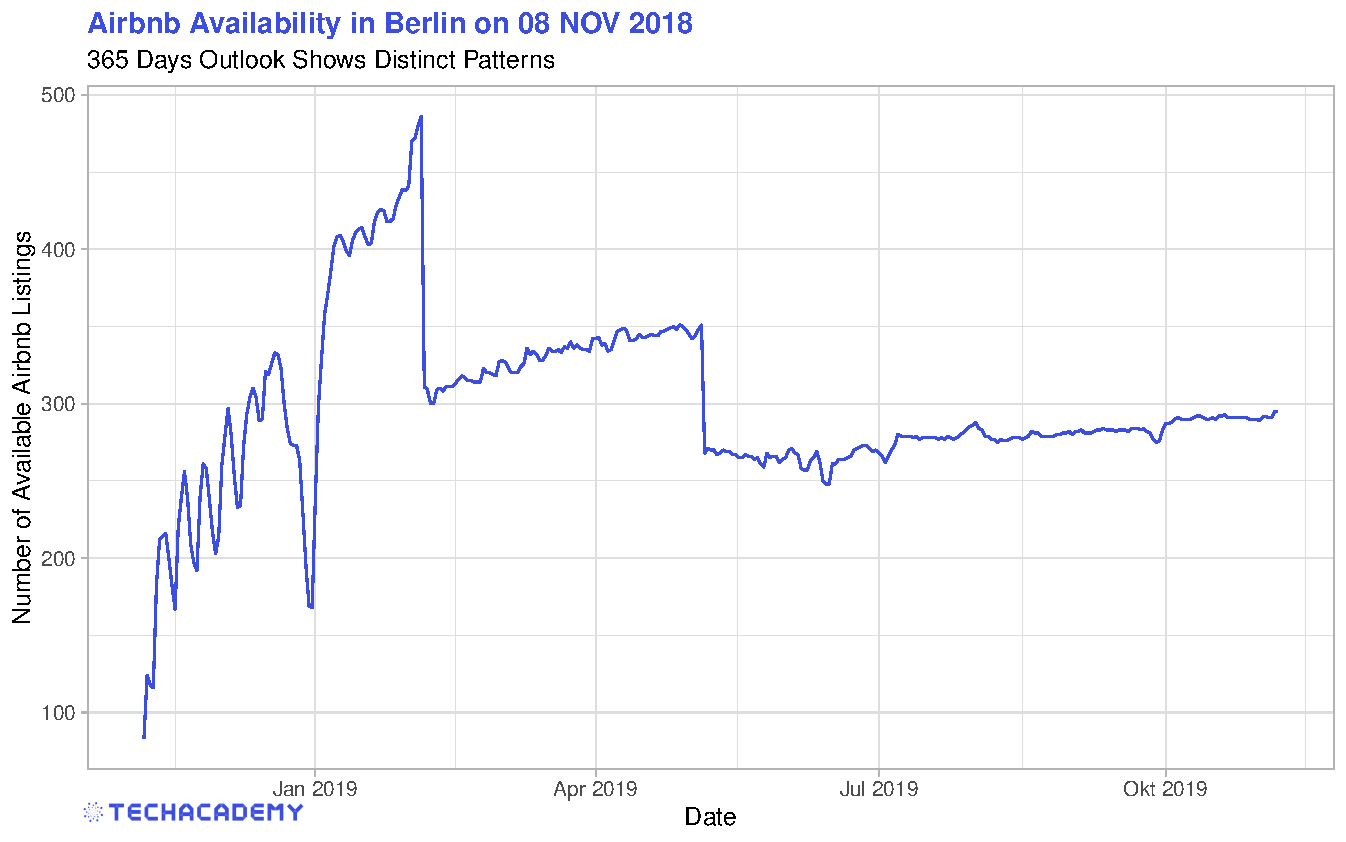
\includegraphics[width=1\linewidth]{plot/1_3_AvailabilityOutlook} \end{center}

The following is a more refined example to show you how you can improve a simple line plot to a more complex and informative plot. The attention of the viewer can be brought to certain patterns this way. But don't get caught up in all the little details, refine your plot to your liking and then move on to the next task. You can always come back to this and play around with the different refinement options.

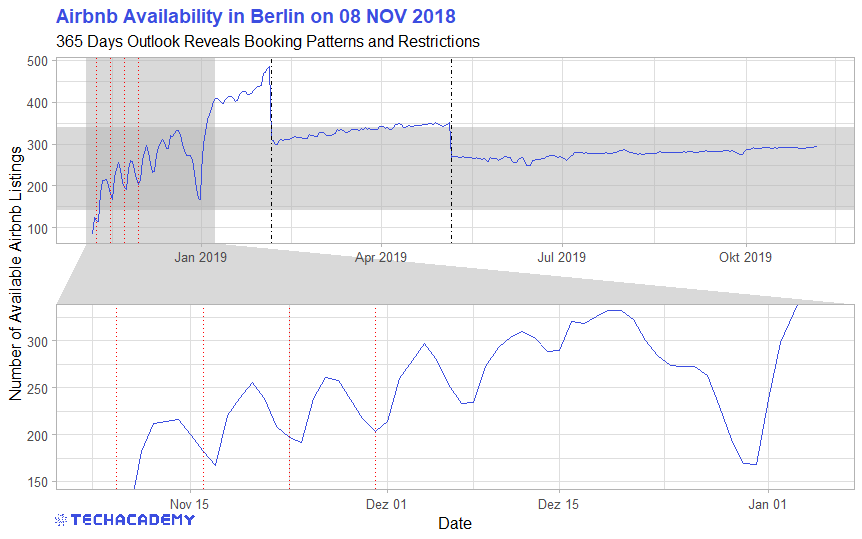
\includegraphics[width=1\linewidth]{plot/1_3_AvailabilityOutlook_advanced}

\begin{tips}r

You can use the base package that includes the function \texttt{plot()} or you could use the more extensive and very flexible graphics package \texttt{ggplot2}.

\end{tips}

\begin{tipsp}p

Having the data in the right format we can now start plotting a simple line graph. For this you can use matplotlib's \texttt{plt.plot()}.

\end{tipsp}

Looking at the line plot, you can see a clear pattern with respect to different dates. There are distinct drops in the availability of the Airbnb apartments. \textbf{One task for your project is to explain the cause behind this pattern.}

\hypertarget{visualize-individual-airbnb-offers-with-the-listings-dataset}{%
\subsection{Visualize individual Airbnb offers with the listings dataset}\label{visualize-individual-airbnb-offers-with-the-listings-dataset}}

After looking at the availability over time using the \texttt{calendar} data set in the first step, we would now like to find out a little more about the price structure of the available apartments. For this we need the \texttt{listings} data set that we can load into the workspace as usual. A closer look reveals that the \texttt{price} and \texttt{cleaning\_fee} columns contain characters and once again need to be cleaned.

Therefore, as in the first task, the dollar sign as well as the comma must be deleted from these columns. Since you use the same procedure for the \texttt{price} and \texttt{cleaning\_fee} columns, a \texttt{for}-loop is recommended here. Implement this loop in a self-written function \texttt{clean\_price()}, so that you save a lot of lines of code, especially in the prediction part.

\begin{tips}r

There are different ways to create this for-loop, so just experiment with what makes most sense to you.

But you definitely want to iterate over all values within one column, so your for-loop function should contain

\texttt{for\ (i\ in\ 1:length(column\_name))}

where ``column\_name'' only acts as a place holder for the variable you want to work on.

\end{tips}

\begin{tipsp}p

Create a list containing the column names of both columns you want to iterate over.

The for-loop body doesn't necessarily need more than one line and might start like this:

\begin{verbatim}
for column_name in column_names_list:
    df[column_name] = train[column_name].str.replace(....
\end{verbatim}

\end{tipsp}

Now that we have cleaned up the data set, we can take a closer look at the price structure of the various neighborhoods. First of all, we would like to know what the average price and the corresponding standard deviation is for each neighborhood. Make a list with the names of the different parts of the city as well as the \texttt{mean} and the \texttt{sd}.

\begin{tips}r

For this, you can again use \texttt{dplyr}-functions like \texttt{group\_by()} or \texttt{summarize()}.

\end{tips}

\begin{tipsp}p

Once again you can use the groupby method to group by neighborhood and apply the aggregation function \texttt{.std()} to get the standard deviations. Similarly, you can use \texttt{.mean()} to get the mean values. Filter both data frames by the price column.

\end{tipsp}

We now want to compare the price distribution for the on average most expensive district with the on average least expensive district. For this, you have to think about the different types of plots that you have gotten to know in your courses and have to find the plot type that is most suited for this type of visualization. Once you have created the diagram, you will probably have to filter out some of the outliers with extremely high prices in order to get a meaningful plot.

\begin{tips}r

In \texttt{ggplot2} graphics, you can easily filter in the plot specifications with \texttt{xlim} or \texttt{ylim}.

\end{tips}

\begin{tipsp}p

One way to find the on average most expensive neighborhood is to simply sort the mean price column in descending order.

For plotting: The Matplotlib documentation is a great source of inspiration with many examples including code that generated them.

\end{tipsp}

On the Airbnb website, the available apartments can be sorted by price and are shown to the customer in the appropriate order. One method to end up higher in this ranking is to quote a low price and a higher cleaning fee. Can we see this behavior in our data set? To figure this out, create an additional column in your data frame with the name \texttt{price\_and\_clean}, in which you add both individual prices. Now examine how the price distribution changes in the two previously examined parts of the city. Compare the price and price + cleaning fee of a district in a diagram. What do you observe?

\hypertarget{merging-of-listings-and-reviewing-the-data-set}{%
\subsection{Merging of Listings and Reviewing the Data Set}\label{merging-of-listings-and-reviewing-the-data-set}}

In the previous part you got to know and visualized the listings data set. However, one important piece of information is not included in this data set: How popular are the individual apartments? We use the number of reviews on Airbnb as a measure of this. This variable could later become very important for price prediction. Fortunately, we have another data set, \texttt{reviews}, in which the apartment ID and the date are saved for each individual review. Our goal now is to count the number of reviews for each individual apartment and to save them. Since we can also find the ID in the listings data set, we can use this variable to merge the two data sets.

First load the new \texttt{reviews} data set into your workspace and take a closer look at it with the familiar functions. Now count the number of reviews per apartment.

\begin{tips}r

This works with the \texttt{table()} function or with \texttt{group\_by()} and \texttt{summarize()}. Note, however, that you still have to convert the result of the \texttt{table()} function into a \texttt{data.frame} format for further processing.

\end{tips}

\begin{tipsp}p

Count the number of reviews per apartament (i.e.~per ``listing\_id'') with the functions you're already familiar with at this point. You can use the groupby argument \texttt{as\_index=False} to avoid setting the column id as index.

\end{tipsp}

Now look at the new data set. Does each ID have exactly one entry with the number of ratings?

To be able to merge the data sets, you have to rename the newly generated variables in the new data set. Name the apartment ID analogous to the \texttt{listings} data set \texttt{id}, as well as the number of reviews \texttt{n\_reviews}.

\begin{tips}r

This can be done with the function \texttt{rename()} from the \texttt{dplyr} package.

\end{tips}

\begin{tipsp}p

Assign the new column names as a list to the \texttt{.column} attribute.

\end{tipsp}

If your data set looks like this, you can merge it with listings:

\begin{center}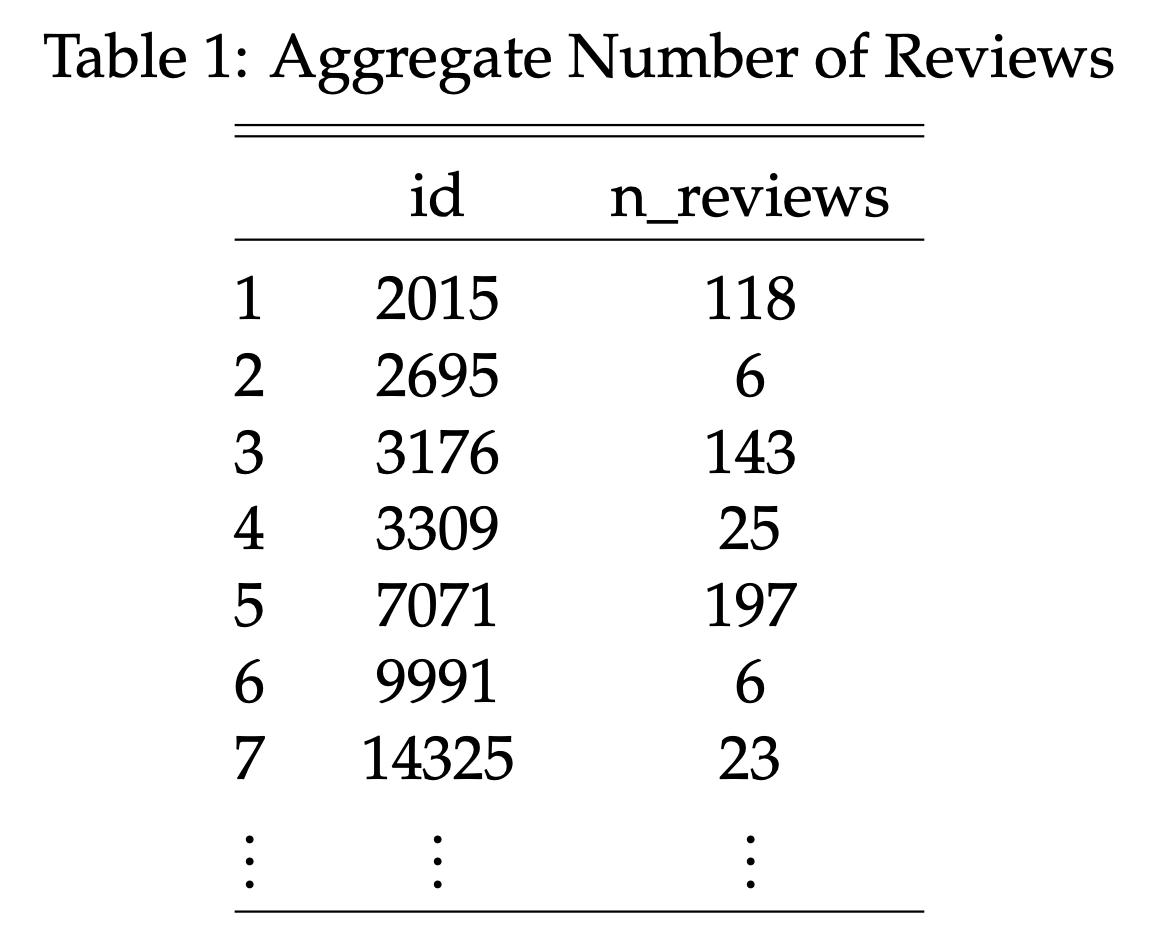
\includegraphics[width=0.4\linewidth]{plot/2_merging_table} \end{center}

\begin{tips}r

You can use the following structure for merging:

\texttt{listings\_reviews\ \textless{}-\ merge(dataset1,\ dataset2,\ by\ =\ ...)}

\end{tips}

\begin{tipsp}p

Merge with \texttt{listings\_reviews=pd.merge(dataframe1,dataframe2,left\_on=...}.

\end{tipsp}

Take a look at the new data set. Is the new variable \texttt{n\_reviews} in the correct data format?

\hypertarget{your-first-barplot}{%
\subsubsection{Your First Barplot}\label{your-first-barplot}}

We now want to take a closer look at a smaller part of the data set: What do the most popular apartments have in common? As an indicator of the popularity of an offer we use the previously generated number of reviews \texttt{n\_reviews}.

Extract the 200 most reviewed apartments. One approach for this is to first sort the data set in descending order according to \texttt{n\_reviews} and then to extract the first 200 entries into a new data set.

Now you can easily visualize the districts in which the 200 most frequently reviewed apartments are located. A bar plot is ideal for this. Feel free to try other types of plots that can be used to best answer this question.

This is what it could look like:

\begin{center}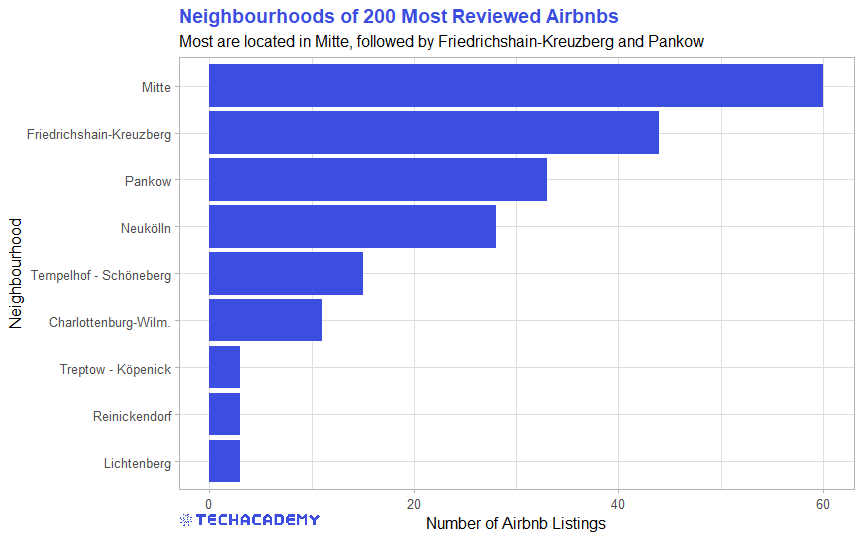
\includegraphics[width=1\linewidth]{plot/3_3_Barplot_MostReviewed} \end{center}

\begin{tips}r

The key commands that you can use for this within \texttt{ggplot()} are \texttt{geom\_bar()} and \texttt{coord\_flip()}.

\end{tips}

\begin{tipsp}p

You can plot bar plots with both pandas and matplotlib.
If you chose to plot with matplotlib, you could use the \texttt{plt.barh()} method. Additionally you might want to use methods like \texttt{.set\_yticks()}, \texttt{.set\_yticklabels()} and \texttt{.invert\_yaxis()}.

If Python throws you an \texttt{AttributeError}, then try working with the \texttt{plt.gca()} method.

\end{tipsp}

\hypertarget{visualization-with-maps}{%
\subsection{Visualization with Maps}\label{visualization-with-maps}}

This part will be the final and most advanced part of the EDA -- but also the most rewarding. Anyone who knows the Airbnb website has probably also seen their map showing the locations of all apartments. We can do the same! The only difference is that our data gives us even more options to show what really interests us!

To reduce complexity, use the smaller data set filtered in the third task with the 200 most frequently reviewed apartments for this task.

We can then place actual objects on the map. Plot the 200 top rated listings on the map. If you have not solved task 3 yet, simply select 200 listings according to other criteria or at random to solve the task. It could look like this:

\begin{center}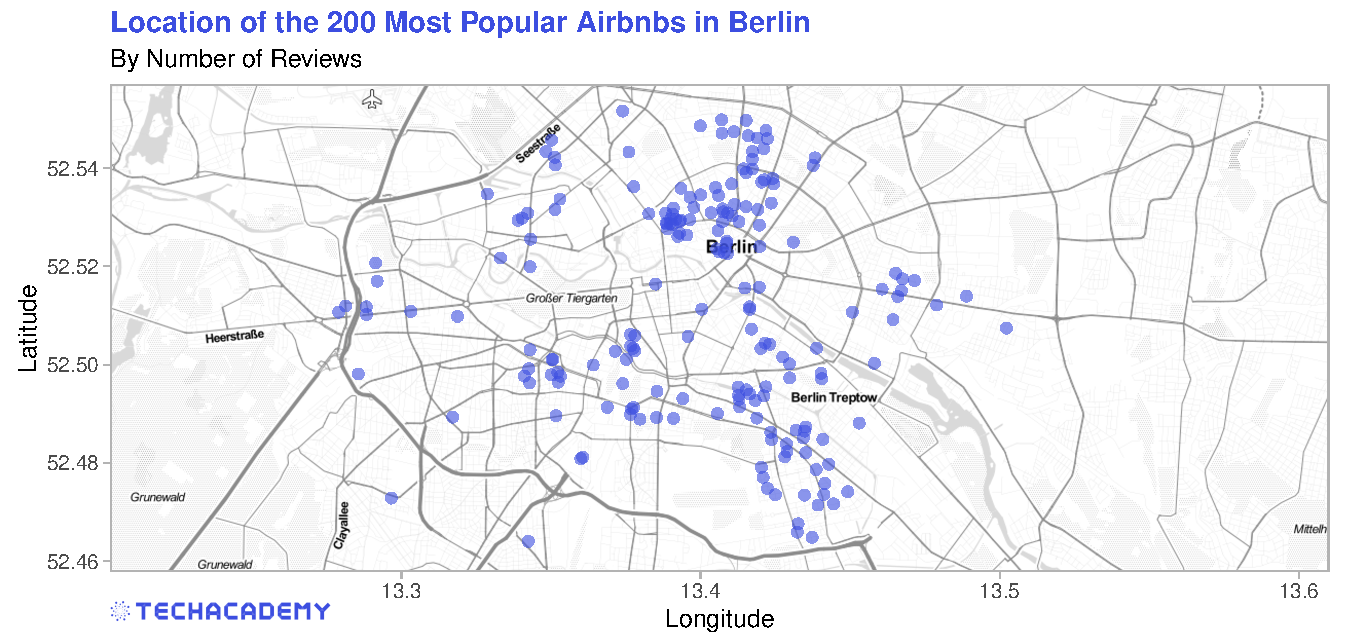
\includegraphics[width=1\linewidth]{plot/4_1_map_top200_simple} \end{center}

\begin{tips}r

There are different ways of creating a map with \texttt{R}, but the following tips will be about the \texttt{ggmap} package.

Before you can download map material via an API interface, you have to define the corners of the map as coordinates.

First define the height and width of the included coordinates. In the next step you can use this to define the exact corners relative to the coordinates in the data set.

\begin{verbatim}
height <- max(...) - min(...)
width <- max(...) - min(...)
\end{verbatim}

You can then define a vector, which you can call \texttt{berlin\_borders}, for example. It is used to define the values for the edges of the map. You can add a small safety margin to the respective minima or maxima of the coordinates. Play around with the factors later to find a good section of the map.

\begin{verbatim}
berlin_borders <- c(bottom = min(listing_top200$latitude) - 0.1 * height,
top = max(listing_top200$latitude) + 0.1 * height,
left = min(listing_top200$longitude) - 0.1 * width,
right = max(listing_top200$longitude) + 0.1 * width)
\end{verbatim}

Then we download the defined map section from the service provider Stamen Maps with the \texttt{get\_stamenmap()} function and save it in an object.

\end{tips}

\begin{tipsp}p

We are going to use yet another library, this one is called Folium. For this task you will need to work with its documentation which you can find online.

Make sure the folium package is installed: You can install it directly from within your notebook by executing \texttt{!pip\ install\ folium}.

Use folium's \texttt{Circle} to draw a circle for each apartment at its location coordinates. You will need to use a for-loop to iterate over all 200 apartments.

\begin{verbatim}
# Initiate the map
m = folium.Map(
    location=[52.5, 13.4],
    tiles='Stamen Toner',
    zoom_start=11
)

# Use a for-loop to plot circles
for lat, long in ... :
    # Your code here

m  # Displays the map
\end{verbatim}

\end{tipsp}

In addition to the coordinates, there is a lot of information about each listing in our data. This time plot the apartments in different colors.

Use the city districts as a distinguishing feature (also to easily see whether the district assignment actually works). It is sufficient if you implement the same plot as before, only with different colors. However, this is an example of how a more advanced plot can look like:

\begin{center}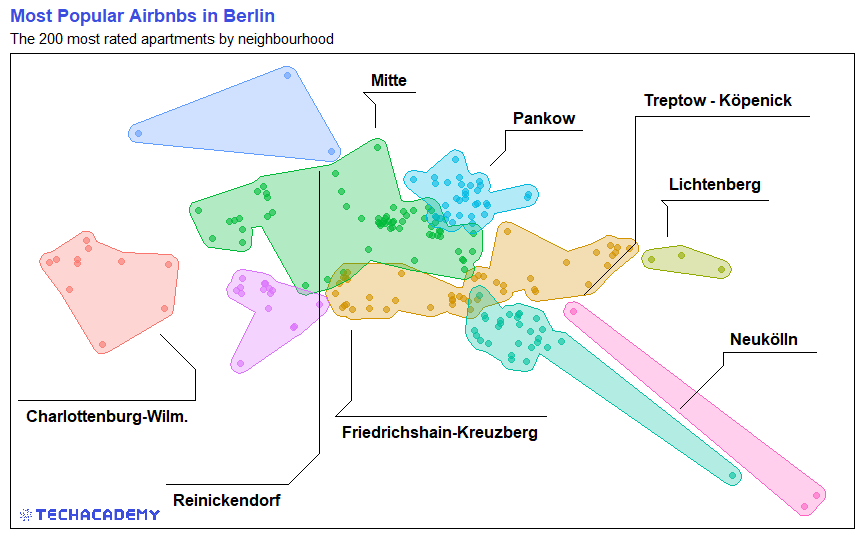
\includegraphics[width=1\linewidth]{plot/4_2_map_top200_by_neighbourhood} \end{center}

\begin{tips}r

This plot was created with \texttt{ggmaps} and the additional package \texttt{concaveman} and its function \texttt{geom\_mark\_hull()}, which draws polygons around a cluster of coordinates.

\end{tips}

\begin{tipsp}p

The plot shown has been created in \texttt{R}. In \texttt{Python} you'll simply color the dots differently for each neighborhood.

The obvious solution for this task would be to filter the data frame by a neighborhood and to create a for loop plotting the circles for that specific neighborhood. Then, repeat this process for all the other neighborhoods using different colors.

This approach would lead to repeating (and thus, bad looking) code: Can you find a better way?

\end{tipsp}

For some analyzes it is easier if you don't just see points, but their distributions on a map. For example, to see where there are many apartments in a small space, you can display the apartment density. It could look like this:

\begin{center}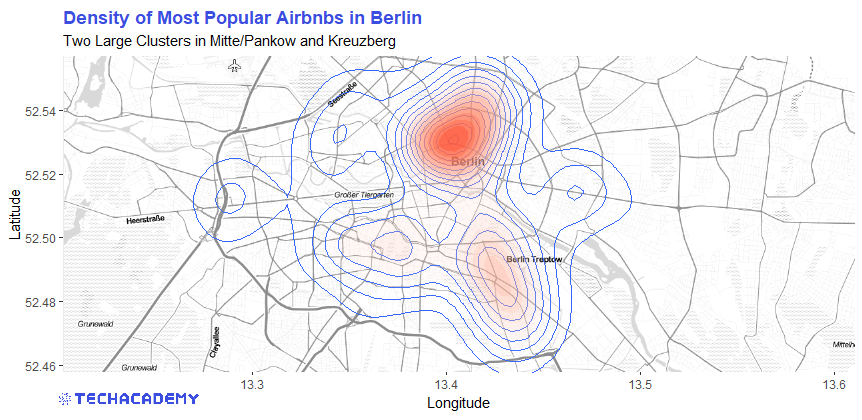
\includegraphics[width=1\linewidth]{plot/4_3_map_top200_density} \end{center}

\begin{tips}r

To create such a two-dimensional density plot you can use the \texttt{geom\_density2d()} and \texttt{stat\_density2d()} packages on the map. If you don't know exactly how the individual arguments should be filled, you can always google for more help.

\end{tips}

\begin{tipsp}p

No hints or tips here - it's up to you to study the documentation for folium's Heatmap and to come up with a (possibly) nice heatmap ;)

\end{tipsp}

Congratulations -- based on your work with basic data transformations and many visualizations, you now have a solid understanding of the Airbnb offers in Berlin. With this, you have now successfully completed the first part of the project! If you are in the beginner group, your minimum requirements are hereby met. Nevertheless, we strongly recommend that you also have a look at the following part. There you'll be developing methods to predict the price of an apartment! Sounds exciting, doesn't it?

\newpage

\hypertarget{price-prediction-application-of-statistical-methods}{%
\section{Price Prediction -- Application of Statistical Methods}\label{price-prediction-application-of-statistical-methods}}

In the previous part you got a feel for the data set. You now know which variables are included and a few characteristic properties of the data set. But so far, we have only visualized the data set. In this section we go a step further and use statistical methods to predict the price of individual Airbnb apartments as accurately as possible.

In order to be able to compare your models at the end, we use a uniform metric according to which we can check the price predictions for accuracy. In our case this is the Root Mean Square Error (\(RMSE\)), i.e.~the root of the average squared difference between the predicted (\(\hat{y}_i\)) and actual value (\(y_i\)):

\[ RMSE = \sqrt{\frac{1}{N}\sum_{i=1}^{N}{(\hat{y}_i-y_i)^2}} \]

The closer the \(RMSE\) is to 0, the better your model predicts prices. In the following, your goal is therefore to reduce the \(RMSE\) of your various models as much as possible through continuous improvements.

We use three different data sets for the following part, which you can find in the subfolder \emph{Full Data Set}. These are based on a much more extensive data set that contains a total of 96 variables for each apartment. We have already done the test / train / validation split of the data so that each group works with the same data sets.

Here is a brief description of what you need each of the data sets for:

\begin{itemize}
\item
  \emph{train.csv} (60 \%): You use this training data set to train your model. The model can learn the relationships between the variables based on the training data set that contains both, the variables needed to predict the prices and also the actual prices themselves.
\item
  \emph{test.csv} (30 \%): With this test data set you can test how well your model predicts the price using data that has not been seen before. This will help you for example with recognizing under- or overfitting.
\item
  \emph{val.csv} (10 \%): We have removed the \texttt{price} variable in this validation data set. At the end you apply your best model to it and send us your predictions for the variable \texttt{price}.
\end{itemize}

We then compare these with the actual values (only known to us) with the help of the \(RMSE\) and will then choose the best model across all groups.

Note that some adjustments are necessary in these three data sets. For example, all price variables are marked with a \$ sign. As before, we need to remove these in order to be able to transform the values to a numeric format. Always keep in mind that you have to apply all transformations to all three data sets, otherwise you will not be able to apply your trained model to the test and validation data sets.

\hypertarget{examine-the-correlation-between-the-variables-train}{%
\subsection{Examine the Correlation Between the Variables (train)}\label{examine-the-correlation-between-the-variables-train}}

First load the \texttt{train.csv} data set from the \emph{Full Data Set} folder into your workspace. Now look at the variable names and the first entries to decide which variables could be useful for predicting the price. Select these (limit yourself to no more than 20 variables at first) plus \texttt{price} and save it in a new data frame.

How are the individual variables related to each other? In other words, to what extent do the variables in the data set correlate with one another? Finding this out is extremely important for deciding which model specification to use later. A good place to start is to create a correlation matrix:

\begin{center}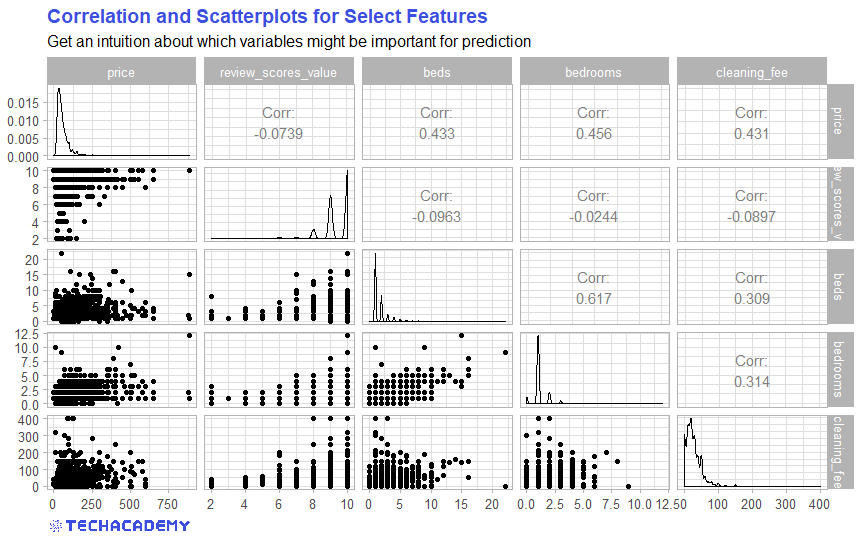
\includegraphics[width=1\linewidth]{plot/5_1_ggpairs} \end{center}

\begin{tips}r

Part of that is function \texttt{cor()} from the base package. Select all numerical variables in your data set with the help of \texttt{sapply()} and create a correlation matrix.

The \texttt{GGally} package with the \texttt{ggpairs()} function provides a very practical plot for visualizing relationships between many variables.

Select the four variables (and \texttt{price}) that you think most influence the price and create a \texttt{ggpairs} plot. Note that the plot quickly becomes illegible and takes a long time to create as soon as you plot significantly more than five variables.

\end{tips}

\begin{tipsp}p

A handy library for plotting correlation matrices is the seaborn library: \texttt{import\ seaborn\ as\ sns}.

Use its pairplot method and pass on the dataframe with the selected columns to visualize distributions and correlations.

Additionally, you may want to plot a heatmap with \texttt{sns.heatmap()} which makes it even easier to see correlations.

\end{tipsp}

Which of your examined variables correlates most with price and which seems to be more independent from price? You now have a first impression over which variables could be important for your model. So let's get to your first price prediction model!

\hypertarget{first-predictions-with-simple-regression-models-train}{%
\subsection{First Predictions with Simple Regression Models (train)}\label{first-predictions-with-simple-regression-models-train}}

Now you can make use of your statistical knowledge. You will need a method with which you can predict the price of an Airbnb apartment for a specific day. A very simple first approach would be to use the average demand as the first prediction. However, this is almost certainly not the best prediction. In this case, your predicted price would be the same over all days and would ignore all factors that influence the price.

Ever heard of linear regression? That would be a much better approach. Now you can use your statistics skills. First set up a model with the dependent variable \texttt{price}. In the previous exercise you examined different variables. Now choose the variable with the highest correlation to price and use that as the only independent variable.

For example, your first regression model could look like this:

\[price_i = \beta_0 + \beta_1 bedrooms_i + \epsilon_i\]

\begin{tips}r

In \texttt{R} you can implement a simple linear regression with the function \texttt{lm()}. You then get the model summary with the \texttt{summary()} function.

\end{tips}

\begin{tipsp}p

Define both dependent (y\_train) and independent (X\_train) variables and clean the data if necessary.

For the next step the X\_train values need to be reshaped \texttt{.values.reshape(-1,1)}.
Note: If you use more then one feature you don't have to reshape your data.

Import \texttt{LinearRegression()} from \texttt{sklear.linear\_model} and train your model using \texttt{LinearRegression().fit()}.

\end{tipsp}

Does your independent variable have a statistically significant impact on apartment price? Probably yes, because we selected the variable most correlated with price. However, if we stick to this very simplified model, we are making a typical mistake: the so-called Omitted Variable Bias (OVB). To put it simply, we neglect (in statistics jargon: ``do not control for'') variables that have a significant influence on the dependent variable. One could suspect that other influencing factors also play a large role in price setting. If we do not include them, the estimate of the effect of \texttt{bedrooms}is biased and thus hardly useful. In our case this is not a big problem for the time being, since we are not interested in causal effects, but rather in the best possible prediction. Your statistics professor would almost certainly object to such a model. Nonetheless, with just a single explanatory variable, this model will not necessarily predict the price well.

One possible solution is to simply include the omitted variables in the model -- how practical that these are already included in the data set. So let's set up a somewhat more extensive model that includes one more variable:

\[price_i = \beta_0 + \beta_1 bedrooms_i + \beta_2 cleaning\_fee_i + \epsilon_i\]

Now compare the results of the two models. Does the larger model explain a higher proportion of the variance in price? In other words, which model shows the higher value for the \(R^2\) measure?

\begin{tips}r

You can easily include such LaTeX tables in your RMarkdown document with the \texttt{stargazer} package:

\begin{center}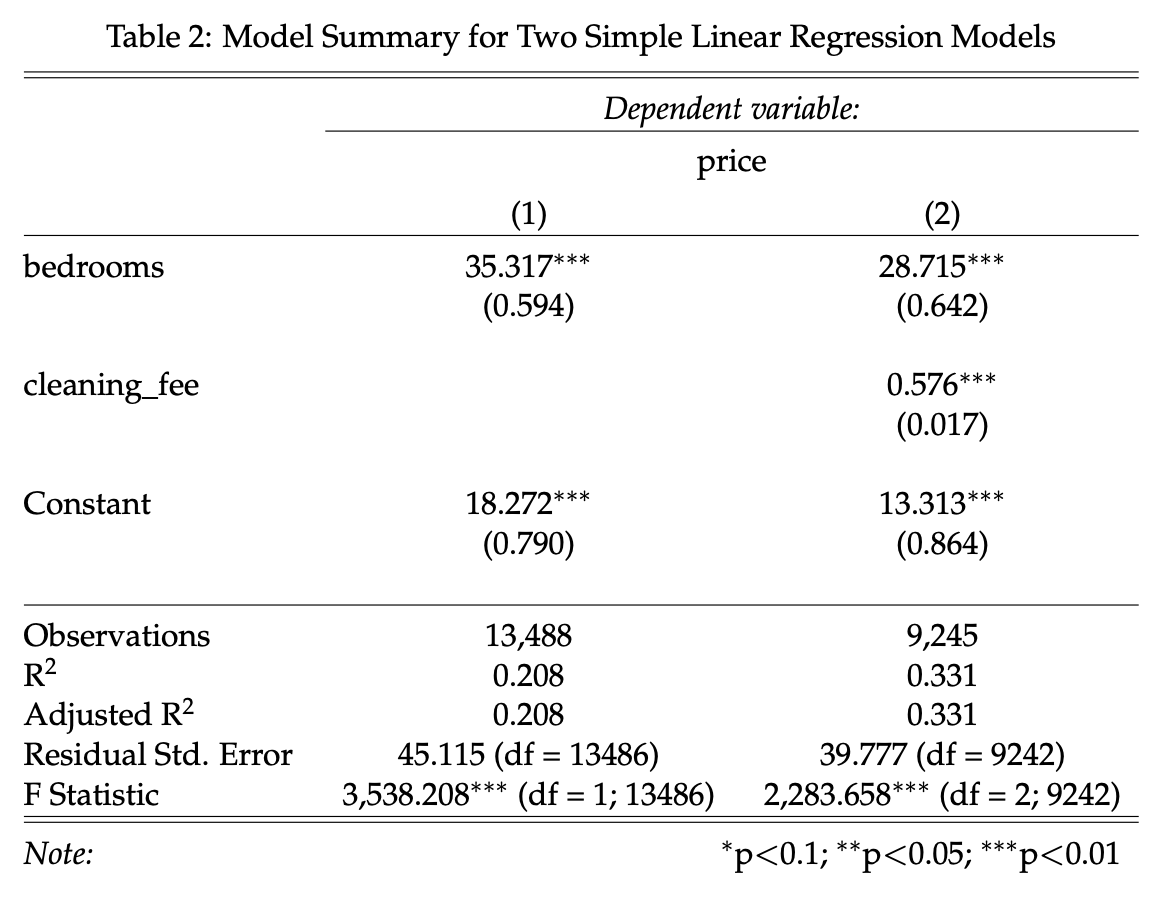
\includegraphics[width=1\linewidth]{plot/5_table} \end{center}

\end{tips}

\hypertarget{from-training-to-testing-making-predictions}{%
\subsection{From Training to Testing -- Making Predictions}\label{from-training-to-testing-making-predictions}}

You have now trained your first model with the training data set. But how well does the model handle data that it has not seen yet? This is a very important test to evaluate the quality of your model.

Has your model only ``memorized'' the existing patterns in the training data set?
Then the relationships from the training data set would not be transferable to the test data set. With so-called overfitting, the model was trained too closely to the training data set and therefore provides poor predictions for unknown data -- for example the data in your test and validation data sets.

On the other hand, there is also the problem of underfitting: Your model has not sufficiently learned the actual relationships between the data and therefore makes poor predictions in the test data set. So it is important to find a balance between the two problems.

Now the distinction between training and test data sets becomes important. As a reminder: we use train data to train a model and the test data to ultimately test the quality of our model.

Now load the data set \texttt{test} in addition to the data set \texttt{train} that you have already used. In order to test your model on previously unseen data, you can apply the model to the test data set.

\begin{tips}r

Use the \texttt{predict} function for this:

\texttt{predicted\_price\ \textless{}-\ predict(your\_saved\_model,\ your\_test\_data\_frame)}

You have now created a vector with all price predictions for the test data set. You can now compare this with the actual values for \texttt{price} from \texttt{test}.

In order to use a uniform comparison metric, please use the following function to measure your prediction accuracy:

\begin{verbatim}
# Function that returns Root Mean Squared Error while ignoring NAs
rmse <- function(actual, predicted) {
sqrt(mean((predicted - actual)^2, na.rm = TRUE))
}
\end{verbatim}

\end{tips}

\begin{tipsp}p

After training, import the data from the \texttt{test.csv} file, define both variables \texttt{X\_test}and \texttt{y\_test}, and create a vector with price predictions applying \texttt{.predict(X\_test)} on your model. Store your prediction in the variable \texttt{predicted\_price}.

Finally, compare your predicted values with the test values:

\begin{verbatim}
from sklearn.metrics import mean_squared_error
# Function that returns Root Mean Squared Error while ignoring NaNs
rmse = mean_squared_error(y_test, predicted_price, squared=False)
\end{verbatim}

\end{tipsp}

Now compare both regression models. Does the larger model have better prediction accuracy, i.e.~a lower \(RMSE\)? Now you have a benchmark for your more advanced models, which you can beat in the next part.

\hypertarget{apply-advanced-machine-learning-algorithms}{%
\subsection{Apply Advanced Machine Learning Algorithms}\label{apply-advanced-machine-learning-algorithms}}

Now that you have created and tested an initial prediction using a simple regression model, you can now apply more advanced methods. The goal is still to get the lowest possible \(RMSE\) when applying the model to the test data set. Now look at at least one other algorithm and then see if that gives you a more accurate prediction (expressed as a lower \(RMSE\)). You can find inspiration for this in the advanced DataCamp courses, which are listed at the beginning of the project guide. There are no limits for you -- you can refine the regression using certain methods (e.g.~LASSO) or set up a random forest model or a neural network. It is usually a good idea to briefly recall the functionality of the respective algorithms and to consider whether this methodology makes sense in this case with a continuous prediction variable.

At this point, a disclaimer is appropriate: Our data set has a substantial part of missing observations (\texttt{NA}) for many variables. Some machine learning algorithms require a complete set of data with no missing values, while others can do well with a smaller number. If you get into trouble about the missing values, check whether you can impute the missing values. Which method is best for imputation depends heavily on your prediction algorithm.

You can also get a noticeable gain in predictive power by modifying existing variables or generating new variables from the data set (``feature engineering''). For example, we could imagine that the distance from an apartment to the city center has a significant impact on the price. However, this variable is not
included in our data set. You can write a simple function that uses the two coordinate variables to calculate the distance to the center of Berlin and appends this to the data set as a new variable.

Always compare the \(RMSE\) of your advanced models with each other, as well as with the benchmark regression model from before.

Did you find your best model? Then predict prices with your winning model as above -- but this time on the validation data set \texttt{val.csv}.

Attach a \texttt{.csv} dataset in the following format with only the two variables \texttt{id} and \texttt{predicted\_price} as an attachment to your project submission.

\begin{tips}r

You can do this by adding the two vectors \texttt{id} and \texttt{predicted\_price} together and saving them as a \texttt{.csv} file.

\begin{verbatim}
submission <- cbind(val$id, predicted_price_val)
write.csv(submission, "submission_<<TEAM NAME>>.csv", row.names=FALSE)
\end{verbatim}

\end{tips}

\begin{tipsp}p

You may need to do some mapping operations between the train.csv data and the predictions to get to the data frame with id and predicted prices.

Similarly as with the \texttt{pd.read\_csv(path/to/file.csv)} method to load data, you can also write data with the \texttt{df.to\_csv(file.csv)} method.

\end{tipsp}

Congratulations! You've made it to the end of your TechAcademy Data Science project. After visualizing the data in the first part, you've also set up predictive models in this section. If you stuck around until this part and managed to code the better part of the exercises, you've definitely earned your certificate! We hope you had fun learning Data Science with this data set and you enjoyed it -- at least the parts where you didn't get stuck forever because of some unexplainable coding error. Don't forget to send your project results and the prediction-csv file you just generated to our project submission email address before the deadline.

\newpage

\hypertarget{excercise-checklist}{%
\section{Excercise Checklist}\label{excercise-checklist}}

This checklist should help you keeping track of your exercises. Remember that you have to hand in satisfactory solutions to at least two thirds of the exercises. If you're part of the beginner track this refers to two thirds of part A (EDA) only. If you're part of the advanced track, you have to hand in at least two thirds of both individual parts A and B. Hence, you cannot hand in 100 percent of the first part and only 50 percent of the second one. You'll need more than 66\% in each one for a certificate. After all, you're not really that advanced if you only did half of it, right?

\textbf{Part A: Exploratory Data Analysis (Beginners + Advanced)}

\begin{enumerate}
\def\labelenumi{\arabic{enumi}.}
\item
  Visualize the available apartments (calendar dataset):

  \begin{enumerate}
  \def\labelenumii{\alph{enumii}.}
  \item
    Transform t/f to boolean values True/False
  \item
    Aggregate data after dates
  \item
    Plot available apartments over time
  \end{enumerate}
\item
  Visualize the listings dataset

  \begin{enumerate}
  \def\labelenumii{\alph{enumii}.}
  \item
    Clean and transform the \texttt{price} and \texttt{cleaning\_fee} columns to numeric values
  \item
    Compute mean and standard deviation of apartment prices for each neighborhood
  \item
    Visualize the price distribution for the most and least expensive district
  \item
    Visualize if \texttt{cleaning\_fee} was used to hide costs
  \end{enumerate}
\item
  Merging of \texttt{listings} and \texttt{review} data set

  \begin{enumerate}
  \def\labelenumii{\alph{enumii}.}
  \item
    Aggregate reviews by \texttt{ID}
  \item
    Merge \texttt{listings} and aggregated reviews data
  \item
    Filter and plot amount of apartments in each district
  \end{enumerate}
\item
  Visualize apartments on map

  \begin{enumerate}
  \def\labelenumii{\alph{enumii}.}
  \item
    Draw a circle for every available apartment on map
  \item
    Colorize each circle according to its districts
  \item
    Draw a 2D-density plot
  \end{enumerate}
\end{enumerate}

\textbf{Part B: Price Prediction Using Statistical Methods ((motivated) Beginners + Advanced)}

\begin{enumerate}
\def\labelenumi{\arabic{enumi}.}
\item
  Visualize feature correlations in a correlation matrix/heatmap
\item
  Regression

  \begin{enumerate}
  \def\labelenumii{\alph{enumii}.}
  \item
    Simple regression model using one variable
  \item
    Improve your model using more features
  \end{enumerate}
\item
  Test your model

  \begin{enumerate}
  \def\labelenumii{\alph{enumii}.}
  \item
    Use test data set to predict prices of the apartments
  \item
    Compare your predictions with the true values
  \item
    Train a new model using a more advanced method, send us your model and the predictions of your best model
  \end{enumerate}
\end{enumerate}

\newpage

\hypertarget{whats-next-in-your-data-science-career}{%
\section{What's Next in Your Data Science Career?}\label{whats-next-in-your-data-science-career}}

At the end of your TechAcademy semester, you've successfully coded your way through a whole Data Science project. You liked what you did and would like bring your skills to the next level? Then this section provides you with many useful resources to deepen your knowledge in Data Science in general or Python and R in particular. The first section is useful for every aspiring Data Scientist, while the two following boxes introduce you to some language-specific resources. If you've come across some other useful materials that we didn't mention here, feel free to contact us -- this list is far from complete!

\hypertarget{data-science-in-general}{%
\subsection{Data Science in General}\label{data-science-in-general}}

\hypertarget{version-control-with-git}{%
\subsubsection*{\texorpdfstring{Version Control with \href{https://github.com/}{Git}}{Version Control with Git}}\label{version-control-with-git}}

If you're serious about data science, you will need Git. Better learn it early and start enjoying and appreciating it before it's too late and you're pressured into learning it on the fly! Every project you do should be versioned with Git. Regardless if you're working alone or with a big group of developers. Regardless if you write ten lines of code or a really complex program. With Git, you can keep track of all your changes. It's like a Dropbox/Google Drive for developers, but way better. Pro-Tip: Get free GitHub Pro as a Student with the \href{https://education.github.com/pack}{GitHub Student Developer Pack}. Besides all the perks of GitHub Pro, you'll also free access to many other great tools. See the respective tutorials on how to set up your Git workflow.

\hypertarget{advice-for-non-traditional-data-scientists}{%
\subsubsection*{\texorpdfstring{Advice for \href{https://blog.shotwell.ca/posts/learning_data_science/}{Non-Traditional Data Scientists}}{Advice for Non-Traditional Data Scientists}}\label{advice-for-non-traditional-data-scientists}}

Important advice from Gordon Shotwell, a former lawyer, on what it takes to have a successful data science career coming from a non-computer science background. Extremely encouraging and helpful read on what you should and shouldn't do to reach that goal.

\hypertarget{learn-from-great-data-scientists-on-kaggle}{%
\subsubsection*{\texorpdfstring{Learn from Great Data Scientists on \href{https://www.kaggle.com/}{Kaggle}}{Learn from Great Data Scientists on Kaggle}}\label{learn-from-great-data-scientists-on-kaggle}}

Kaggle is a platform that hosts data science challenges. The great thing about it is that you can browse through many clever solutions to tricky machine learning tasks. And of course, you can also join the competition and measure your predictions with others. There are plenty of both Python and R notebooks.

\hypertarget{r}{%
\subsection{R}\label{r}}

\begin{tips}r

\textbf{Install R and RStudio Locally}

RStudio.Cloud is great for getting started with R without having to worry about installing anything locally. Sooner or later you will have to install everything on your own computer. Here's a \href{https://www.datacamp.com/community/tutorials/installing-R-windows-mac-ubuntu}{DataCamp tutorial} on how to do that.

\textbf{Version Control with Git}

RStudio has a nice interface that lets you enjoy the perks of Git without ever having to touch the command line -- sounds great, does it? Learn how to set up the Git \& R workflow with \href{https://happygitwithr.com/}{Happy Git with R}.

\textbf{\href{https://www.r-graph-gallery.com/}{R Graph Gallery}}

Get inspiration to take your plotting to the next level. Includes code to reproduce the plots.

\textbf{Follow the R Master Himself and the R Community}

Hadley Wickham was and continues to be extremely influential on the development of R and its rise to one of the most popular data science languages. He's behind many tools that we taught you in this semester, especially the tidyverse (including great packages such as ggplot2 and dplyr). Follow him \href{https://twitter.com/hadleywickham}{on Twitter} to get great R advice and keep up to speed with everything new to R. Following the many people behind R (not only Hadley) is a great way for acquiring deeper understanding of the language and its developments.

\textbf{Join the \href{https://www.meetup.com/r-frankfurt/}{Campus useR Group in Frankfurt}}

There's a quite active R community in Frankfurt that meets once a month. It's open for students, professors, industry practitioners, journalists, and all people that love to use R. In those meetings, you'll hear about other's work, discuss new developments, and ask questions.

\textbf{Listen to R Podcasts}
Another great way to easily keep up with new developments in the Data Science/R community. Check out
\href{http://nssdeviations.com/}{Not So Standard Deviations} or \href{https://r-podcast.org/}{the R-Podcast}

\end{tips}

\hypertarget{python}{%
\subsection{Python}\label{python}}

\begin{tipsp}p

\textbf{Install Python Locally}

Until now you've only programmed using JupyterHub on the TechAcademy Server. A next step would be to install Python and Jupyter locally on your computer. This \href{https://docs.anaconda.com/anaconda/install/}{link} contains the necessary information on how to install the software on Windows, iOS or Linux.

\textbf{Choosing the Right Editor}

Using Jupyter is especially useful for short data analyses. But sometimes you want to write longer scripts in Python. In these cases, it is often more convenient to use a code editor instead of Jupyter. \href{https://realpython.com/learning-paths/perfect-your-python-development-setup/}{This tutorial} highlights the positive aspects of such an editor and how to choose the right one for you. Pro Tip: Also check out the other tutorials on \href{https://realpython.com/}{Real Python}.

\textbf{\href{https://python-graph-gallery.com/}{Python Graph Gallery}}

Get inspiration to take your plotting to the next level. Includes code to reproduce the plots.

\textbf{More Advanced Python Concepts}

You know the basic data structures in Python like lists and dictionaries. What are the next steps to improve your knowledge? \href{https://book.pythontips.com/en/latest/index.html}{This website} gives good explanations for slightly more advanced concepts which can be very useful from time to time.

\textbf{A Deeper Understanding}

If you want to get a deeper understanding of the Python programming language and into typical algorithms which are used in the field of Data Science, this \href{https://github.com/ab-anand/py-books/blob/master/Data\%20Science\%20from\%20Scratch-\%20First\%20Principles\%20with\%20Python.pdf}{free book} can be a good starting point.

\textbf{Writing Beautiful Python Code}

``My code doesn't look nice, but it works!''
This might work for yourself, but often you will work on code with other people. But even if you're just coding for yourself it's a good idea to follow the PEP8 style guide. It's a useful convention on how to structure and code in Python. You'll find useful resources for PEP8 \href{https://realpython.com/python-pep8/}{here} and \href{https://www.python.org/dev/peps/pep-0020/\#id2}{here}.

\textbf{Listen to Python Podcasts}

When you don't have time for books you can listen to \href{https://talkpython.fm/home}{Talk Python} or the \href{https://www.pythonpodcast.com}{Python Podcast}.

\end{tipsp}

  \bibliography{book.bib,packages.bib}

\end{document}
